% ===============================
% Shed setup
% ===============================
\newpage
\section{Experiment set-up}
\label{sec:shedsetup}

Since 2003 the K\"onig lab studies a wild population of house mice in a barn, where mice can leave and enter freely.

The barn is located in a forest near Illnau (Switzerland) and consist of a single room with an area of 64m$^2$ (12.8m x 5.75m). Stable plastic walls (height \textasciitilde50cm) divide the area into four segments and an entry space. Small transit holes in the dividers ensure access to the different segments (see figure~\ref{fig:shedschema}).

The entry area provides workspace for the researchers and is used to store tools and material. Furthermore, the central computer for the data collection system (see section \ref{subsec:collectspatialpos}) is placed in this area.

The 40 artificial nestboxes (see figure~\ref{fig:artNestbox} for a schematic model) are distributed evenly in the four sectors (see figure~\ref{fig:shedschema} for the current positioning of the boxes) along with some plastic pipe structures, bricks, smaller plastic walls and shelters to structure the environment (see figure~\ref{fig:shedoverview}). These structuring elements ensure the existence of several territories, and provide hideouts for the subordinate mice.

\begin{figure}[htpb]
\begin{center}
  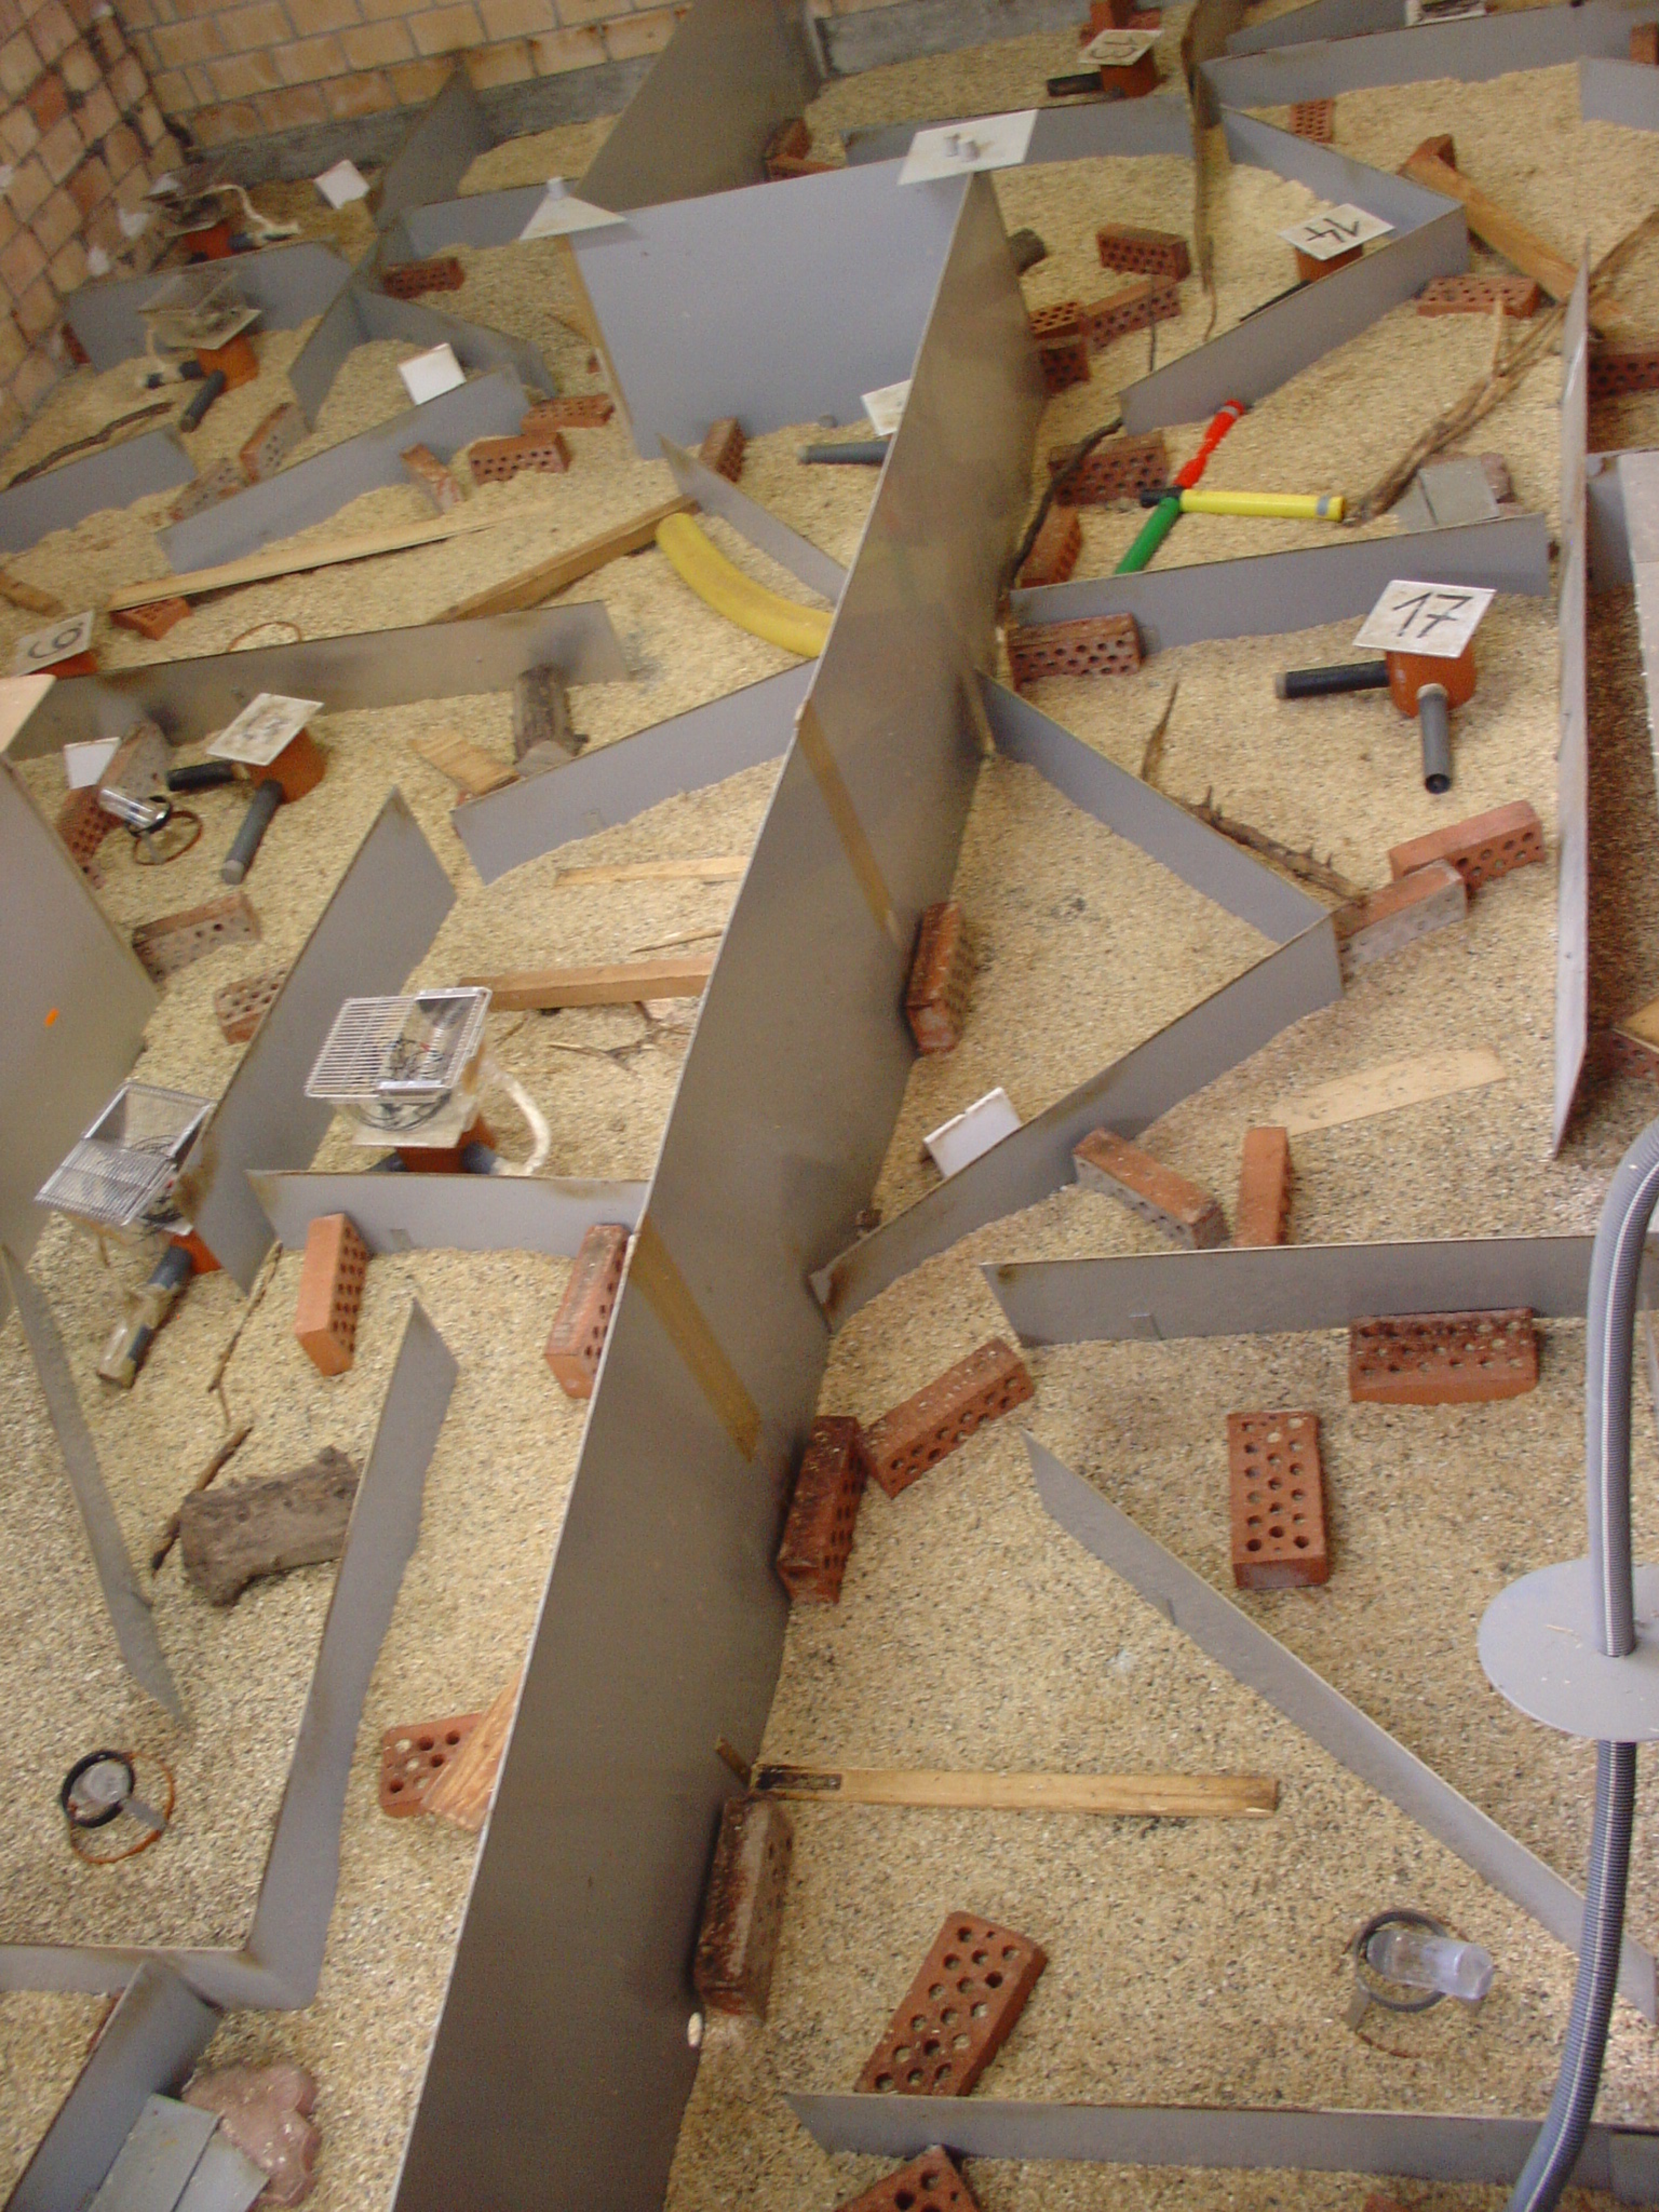
\includegraphics[width=0.7\textwidth]{assets/pdf/shed_overview.pdf}
  \caption[Interior of the barn]{Overview of the interior of the barn. Visible are the artificial nestboxes labeled with the box number on the white cover panel, the grey colored sector dividers and the accessory elements to structure the area.}
  \label{fig:shedoverview}
\end{center}
\end{figure}

\begin{sidewaysfigure}[htpb]
  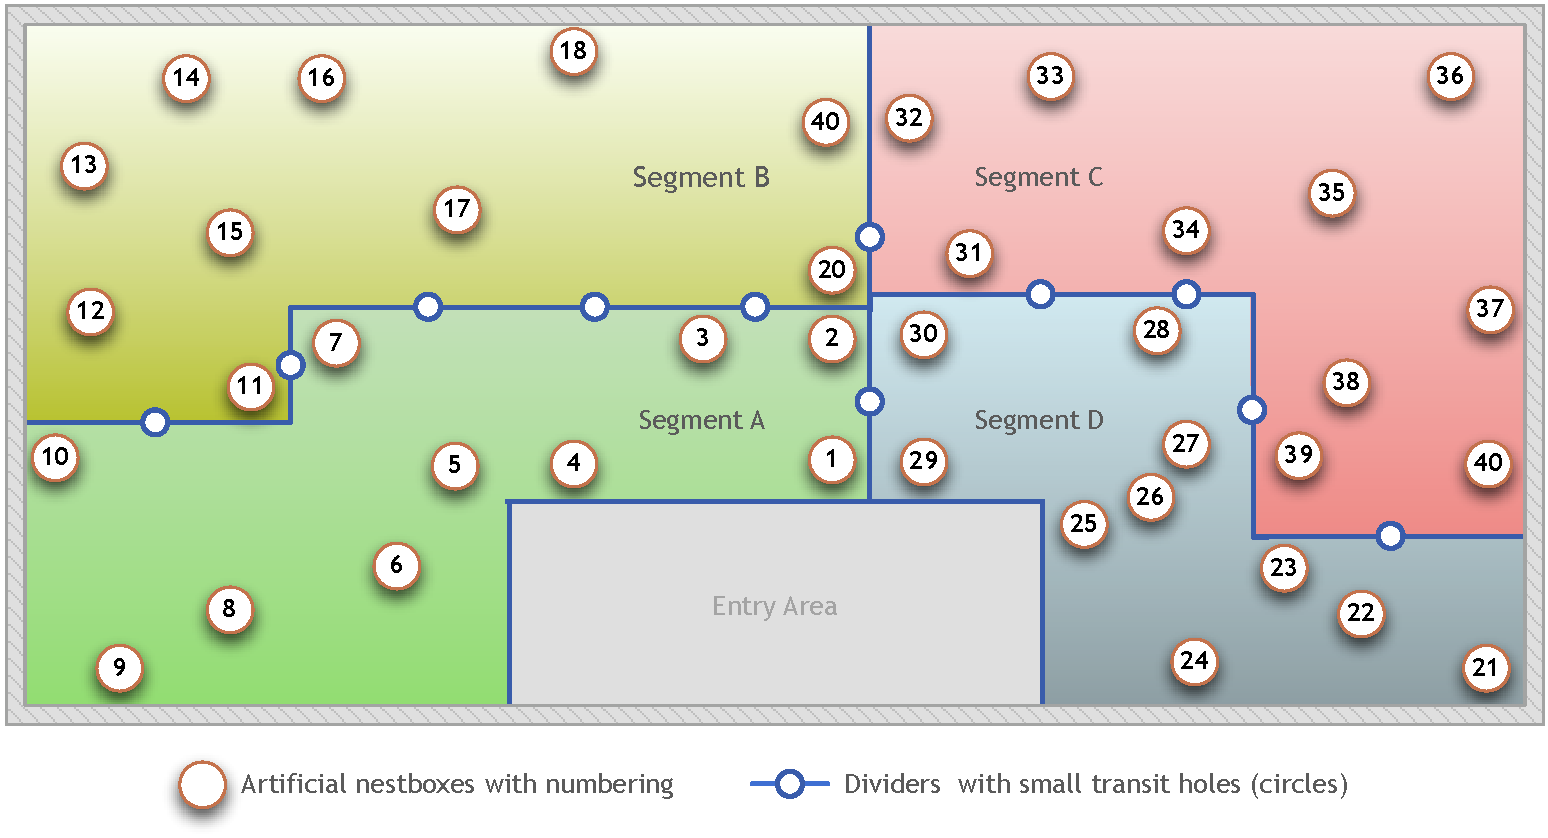
\includegraphics[width=\textwidth]{assets/pdf/shed_schema.pdf}
  \caption[Schema of the barn]{Schema of the barn including the box positions and the plastic walls dividing the area in the four segments. }
  \label{fig:shedschema}
\end{sidewaysfigure}